\section{Кинематика твердого тела}

\begin{to_def} 
    \textit{Абсолютно твёрдым телом}\footnote{
        Для краткости просто \textit{твёрдое тело}.
    } назовём множество такое, что
    $$
         \forall i, j, t:
         \hspace{0.5cm} |\vc{r}_i(t) - \vc{r}_j(t)|=\const.
     $$ 
\end{to_def}

Точка $O$ это полюс. Во-первых перенесем начало координат в $O$. Введём систему координат $O_{\xi\nu\zeta}$ связанную с телом, -- тело относительно неё не движется.
% \textit{Поступательное движение} -- 
% \textit{Вращательное движение} --
$$
    \vc{r} = \vv{OA}, \, \vc{\rho} = \vv{OA} = \const \text{ в $O_{\xi\nu\zeta}$},
    \hspace{0.5cm} \Rightarrow \hspace{0.5cm} 
    \vc{r}(t) = R(t) \vc{\rho}.
$$

% \begin{minipage}[t]{0.45\textwidth}
% \begin{align*}
%     \text{Точка:} \hspace{0.5cm} 
%     \vc{r} \in \mathbb{R}^3, \hspace{0.5cm} n=3 \\
%     \vc{v} \\
%     \vc{\mathrm{w}}
% \end{align*}
% \end{minipage}
% \hfill
% \begin{minipage}[t]{0.45\textwidth}
% \begin{align*}
%     \text{Твёрдое тело:} \hspace{0.5cm} 
%     \vc{r}, R \in \mathbb{R}^3 \times SO(3), \hspace{0.5cm} n=6 \\
%     \vc{\omega} \\
%     \vc{\varepsilon} 
% \end{align*}
% \end{minipage}
\subsection{Углы Эйлера}

\begin{wrapfigure}{r}{0.25\textwidth}
  \begin{center}
        \vspace{-10 mm}
        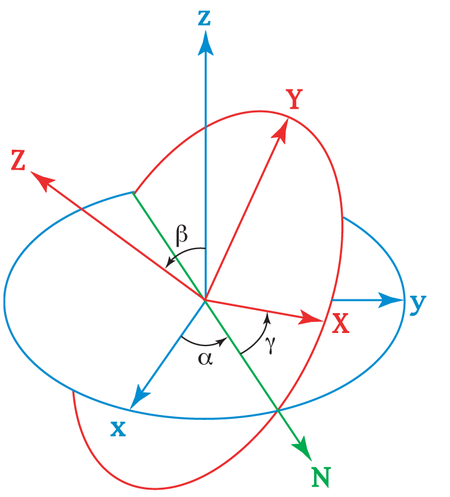
\includegraphics[width=0.9\linewidth]{img/eu_angles.png}
  \end{center}
    \caption{Углы Эйлера}
\end{wrapfigure}

Ортогональность матрицы $R$ даёт возможность описать её тремя независимыми параметрами. Один из вариантов сделать это -- углы Эйлера. 

Пусть начальная ПДСК $(x, y, z)$, а конечная -- $(X, Y, Z)$, при чём $xy \cap XY = ON$ -- линия узлов.
\begin{align*}
    1) \hspace{0.25cm}  \alpha &\colon Ox \to ON, &\text{ угол \textit{прецессии}}; \\
    2) \hspace{0.25cm}  \beta  &\colon Oz \to OZ, &\text{ угол \textit{нутации}}; \\
    3) \hspace{0.25cm}  \gamma &\colon OX \to ON, &\text{ угол \textit{собственного вращения}}.
\end{align*}
Повороты системы на эти углы называются прецессия, нутация и поворот на собственный угол (вращение). 

\phantom{42}

\noindent
\textbf{Матричная запись углов Эйлера}:
\begin{equation*}
    R_Z(\alpha) = \begin{pmatrix}
        \cos \alpha & - \sin \alpha & 0 \\
        \sin    a & \cos\alpha & 0 \\
        0 & 0 & 1\\
    \end{pmatrix},
\end{equation*}
и,
\begin{equation}
    R_X(\beta) = \begin{pmatrix}
        1 & 0 & 0 \\
        0 & \cos \beta & -\sin \beta \\
        0 & \sin \beta \cos \beta \\
    \end{pmatrix},
    \hspace{1cm} 
    R_Z (\gamma) = \begin{pmatrix}
        \cos(\gamma) & - \sin \psi & 0 \\
        \sin \gamma & \cos \gamma & 0\\
        0 & 0 & 1
    \end{pmatrix}.
\end{equation}

\subsection{Основные теоремы о конечных перемещениях твёрдого тела}


Далее бездоказательно приведём некоторые основные теоремы о конечных перемещениях твёрдого тела.

\begin{to_thr}[Теорема Эйлера]
     Произвольное перемещение твердого тела, имеющего неподвижную точку, можно осуществить посредством вращения вокруг некоторой оси, проходящей через эту точку. 
\end{to_thr}

\begin{to_thr}[Теорема Шаля]
     Самое общее перемещение твердого тела разлагается на поступательное перемещение, при котором произвольно выбранный полюс переходит из своего первоначального положения в конечное, и на вращение вокруг некоторой оси, проходящей через этот полюс. Это разложение можно совершить не единственным способом, выбирая за полюс различные точки тела; при этом направление и длина поступательного перемещения будут изменяться при выборе различных 
полюсов, а направление оси вращения и угол поворота вокруг нее не зависят от выбора полюса. 
\end{to_thr}

\begin{to_thr}[Теорема Моцци]
\label{thr_moz}
     Самое общее перемещение твердого тела является винтовым перемещением.
\end{to_thr}

\begin{to_con}[Теорема Бернулли-Шаля]
     Самое общее перемещение плоской фигуры в своей плоскости есть либо поступательное перемещение, либо вращение вокруг точки. Эта точка называется центром конечного вращения.
\end{to_con}

%%%%%%%%%%%%%%%%%%%%%%%%%%%%%%%%%%%%%%%%%%%%%%%%%%%%%%%%%%%%%%%%%%%%%%%%%%%%%%%%%%%
\subsection{Скорости и ускорения точек твердого тела в общем случае движения}
%%%%%%%%%%%%%%%%%%%%%%%%%%%%%%%%%%%%%%%%%%%%%%%%%%%%%%%%%%%%%%%%%%%%%%%%%%%%%%%%%%%

Проведём два вектора $\vc{r}_A, \vc{r}_O$:
$$
    \vc{r}_A = \vc{r}_O + \vc{r} = \vc{r}_O + R(t) \vc{\rho}
    \hspace{0.5cm} \overset{d / dt}{\Rightarrow} \hspace{0.5cm} 
    \vc{v}_A = \vc{v}_O + \dot{R} \rho = \vc{v}_O + \dot{R} R^{-1}\vc{r}
$$
но,
$$
    RR\T = E, \dot{R} R\T + R \dot{R}\T = 0, \dot{R} R\T = - R \dot{R}\T,
    (\dot{R} R^{-1})\T = - \dot{R} R^{-1}.
$$
То есть $\dot{R} R^{-1}$ кососимметрична. Тогда пусть
$$
    \dot{R} R^{-1} = \Omega = \begin{pmatrix}
        0 & -\omega_z & w_y \\
        w_z & 0 & -\omega_x \\
        -\omega_y & \omega_x & 0\\
    \end{pmatrix}
    % матрицу
$$
Таким образом мы доказали следующую теорему.

\begin{to_thr}[формула Эйлера]
\label{eq_euler}
    Существует единственный вектор\footnote{
        Псевдоветор же, нет?
    } $\vc{\omega}$, называемый \textbf{угловой скоростью тела}, с помощью которого скорость $\vc{v}$ точки тела может быть представлена в виде
    \begin{equation}
        \vc{v}_A = \vc{v}_O + \vc{\omega} \times \vc{r}
        \hspace{0.5cm} \text{--} \hspace{0.5cm} \text{\textbf{формула Эйлера}.}
    \end{equation}
\end{to_thr}


Тогда, например, при постоянном радиус векторе верно, что
$$
    \vc{v}_A = \frac{d \vc{a}}{dt} = \vc{\omega} \times \vc{a},
    \hspace{0.5cm} \text{при условии $a = \const$}.
$$
Можно вывести ускорение точки твёрдого тела
\begin{align*}
    \vc{\mathrm{w}}_A &= \vc{\mathrm{w}}_O + \frac{d \vc{\omega}}{dt} \times \vc{r} + \vc{\omega} \times \frac{d \vc{r}}{dt}, \\
    \vc{\mathrm{w}}_A &= \vc{\mathrm{w}}_O + \vc{\varepsilon} \times \vc{r} + \vc{\omega} \times \left(\vc{\omega} \times \vc{r} \right)
    \hspace{0.5cm} \text{--} \hspace{0.5cm} \text{\textbf{формула Ривальса},}
\end{align*}
где $\vc{\varepsilon} = d \vc{\omega} / d t$ -- \textit{угловое ускорение}.



\subsection{(-) Частные случаи.}

Оставим частные случаи в покое.
% Вращение твердого тела вокруг неподвижной оси. 
% Движение вокруг неподвижной точки. 
% Плоское движение тела. 

\subsection{Кинематические инварианты и кинематический винт}

Вернемся к общему случаю движения твёрдого тела. В \eqref{eq_euler} угловая скорость $\vc{\omega}$ точки $P$ инвариантна к выбору точки, соответственно $\omega^2$ -- \textit{первый кинематический инвариант}. Домножив \eqref{eq_euler} скалярно на $\vc{\omega}$, получим, что $I_2 = (\vc{v} \cdot \vc{\omega})$, -- \textit{второй кинематический инвариант}.

Сейчас легко доказать thr. \eqref{thr_moz}, точнее надо показать существование такой прямой $MN$, все точки которой имеют скорости, $\parallel \vc{\omega}$.

Выберем некоторый полюс, $O$, со скоростью $\vc{v}_O$ и угловой скоростью $\vc{\omega}$. Тогда верно, что
$$
    \vc{v}_O + \vc{\omega} \times \vv{OS} = p \vc{\omega}, \hspace{0.5cm} (p \neq 0).
$$



